\documentclass[twocolumn]{revtex4}
\usepackage{graphics,graphicx,epsfig,amsmath,multirow,gensymb,commath,textcomp,natbib,blindtext,tabularx,array,makecell,threeparttable,amssymb,relsize,csquotes}
\usepackage{listings}
\usepackage[a4paper, left=1.85cm, right=1.85cm, top=1.85cm, bottom=1.85cm]{geometry}   
\usepackage[normalem]{ulem}
\newcommand{\squeezeup}{\vspace{-2.5mm}}

\usepackage{lipsum}

\def\bibsection{\section*{\refname}} 
\renewcommand{\thesubsection}{\alph{subsection}}

\renewcommand\theadalign{bc}
\renewcommand\theadfont{\bfseries}
\renewcommand\theadgape{\Gape[4pt]}
\renewcommand\cellgape{\Gape[4pt]}

\begin{document}

\textheight=26.385cm
%Change textheight as the last resort...

\title{Constraining the geometry of the Universe using Type Ia supernovae and statistical methods}
 
\author{Jacky Cao, Group C3, Physics Problem Solving \\ Date of report: 28/02/2018}

\begin{abstract}              
Type Ia supernovae have the unique trait of being standard candles, their light curves can be used in cosmology to calculate and constrain cosmological parameters. In observing Type Ia supernovae and fitting model light curves to such data one can attempt to derive such values. We have monitored, collected, and analysed data for supernova explosions over a period of 34 days. A $16''$ and a $0.5$ m telescope situated in Durham and La Palma was used for this project. After calculating the magnitudes for a Type Ia (2017hhz) and Type Ia-91bg (2017hle) supernova object, we fitted template light curves with the Python program, \textit{SNooPy}. The quality of fit for the program's \texttt{fit()} function was deemed to be acceptable in accordance to the average reduced $\chi^2$ values calculated for the B and V photometric bands, $\chi^2_{\nu,B} \approx 1.38$ and $\chi^2_{V,\nu} \approx 2.95$ - a good fit requiring $\chi^2_{\nu} \approx1$. The distance modulus to the supernova 2017hhz was calculated by SNooPy to be $36.121\pm0.106$ mag, using this value we were able to compute $H_0=70\pm20$ km s$^{-1}$ Mpc$^{-1}$. However, the quoted error negates the meaning of $H_0$ as it is too large of an uncertainty. In improving the accuracy and uncertainties we suggest that more observations of the supernovae were required, and constraining values should be used for the parameters in SNooPy's templates.
\end{abstract}

\maketitle

\vspace{-3ex}
\section{Introduction and Theory} 
\vspace{-2ex}
In cosmology, one can argue that one of the most important observable events are supernova explosions. As a massive main sequence star runs out of nuclear fuel to burn, the equilibrium configurations which initially provided structure will cease to exist. What follows is a cataclysmic supernova explosion \cite{longair}. 

We can generally class supernova explosions into two separate groups, Type I and Type II supernovae. The main distinction arises due to the fact that Type I's have an optical spectra which contains no Balmer hydrogen features, whilst Type II supernovae do contain this hydrogen feature \cite{mod_ast}. 

Within these two subclasses there are further divisions which can be characterised through their spectra and through features as found in their light curves \cite{obs_phys_class_sn}. Light curves are a way to show the evolution of a supernova's magnitude as time passes. For example, with two of the subclasses of Type II supernovae, Type II-L and Type II-P, they can be classed from features of their light curves. For a Type II-L supernova there is a rapid linear decrease in magnitude, and with a Type II-P we see a constant magnitude after maximum \cite{mod_ast}.

For the application of supernovae in cosmology, we must turn to the variety of Type Ia.

\vspace{-3ex}
\subsection{Type Ia Supernovae}
\vspace{-2ex}
It is accepted that the light curves of Type Ia supernovae are generally homogeneous \cite{posn}, this means that they can be utilised as standard candles therefore allowing us a measure of cosmic distance. 

Their homogeneity arises due to the mechanism behind the explosion. The progenitor system for Type Ia's consist of a binary system with a primary white dwarf and secondary star which has a mass close towards the Chandrasekhar limit of $1.4 M_{\odot}$ \cite{mod_ast, posn}. The white dwarf will accrete matter from it's companion until it itself reaches the critical mass limit. After this point we would then expect the primary star to collapse into a neutron star, however this is not what happens. Instead, we find that a supernova explosion occurs. An event which arises due to a massive disruption to the star's internal structure by a large amount of energy. [[give a rough value]]

It is currently understood that as the white dwarf accretes matter it heats up and produces thermonuclear energy. This energy is achieved in the stellar interior at a temperature of $10^9$ K, as a result a disruption to the electron degeneracy pressure takes place. The star becomes gravitationally unstable from the nuclear energy and a total collapse into a neutron star is prevented \cite{longair, posn}.

This particular mechanism can be used to explain the standard profile of Type Ia light curves. Using these plots, the maximum B band photometric magnitude can be obtained with the following equation,
\begin{equation}
M_{\max}(B)=-21.726+2.698\Delta m_{15}(B),
\end{equation}

where $\Delta m_{15}(B)$ is the decline rate parameter or Phillips' parameter \cite{high_en_astro}. This is defined as the mean rate of decline of the B band light curve from peak light to 15 days after the maximum \cite{abs_phil}. This parameter relates the apparent magnitude to time and provides a way to compare and contrast different Type Ia supernovae. 

With values for the absolute magnitude of Type Ia supernovae and with values of their redshift obtained from spectroscopic observations, the distance to these objects can then be calculated using the following equation, 
\begin{equation}
\mu = 5 \log_{10}(d) - 5,
\end{equation}

where $\mu$ is the distance modulus and can be defined as the absolute magnitude of supernova subtracted from it's apparent magnitude, and we define $d$ is the distance to the supernova in parsecs \cite{mod_ast}. 

From data sets of Type Ia supernovae we can easily employ them to calculate the geometry of the universe. But before that, we must first understand what cosmological parameters are and how they can be constrained.

\vspace{-3ex}
\subsection{Cosmological Parameters}
\label{sec:cosmo_parameters}
\vspace{-2ex}
At large cosmological distances, the appearance of objects will be affected by the spacetime which it travels through. If we therefore wanted to describe the geometrical properties of the universe, we would require to solve Einstein's general theory of relativity. From \textit{An Introduction to Modern Astrophysics} \cite{mod_ast} we can build the framework required to calculate and compute cosmological parameters. 

If we solve Einstein's field equations for an isotropic, homogenous universe a description of the evolution of the universe can be obtained in the form of a differential equation which is also known as the Friedmann equation. In the 1922 form of the equation, a non-static universe is accounted for,
\begin{equation}
\Big[ \Big( \frac{1}{R} \frac{dR}{dt} \Big)^2 - \frac{8}{3} \pi G \rho \Big] R^2 = -k c^2,
\label{eqn:1922_friedmann}
\end{equation}

where $R(t)$ is the scale factor, $G$ the gravitational constant, $\rho$ is the mass density, $k$ is a parameter which describes the shape of the universe, and $c$ is the speed of light in a vacuum.

$k$ can be defined as a constant which is equal to $-1$ for a negatively curved universe, $0$ for a spatially flat universe, and $+1$ for a positively curved universe \cite{longair}. 

Separate work performed by Einstein eventually led to a cosmological constant $\Lambda$ being introduced in the Friedmann equation. This was included in the form of $\tfrac{1}{3}\Lambda c^2$ within the square brackets of the left hand side of Equation \ref{eqn:1922_friedmann}. Whilst Einstein included this term to account for his static and closed universe, as a consequence of observations which implied an accelerating universe, astronomers in the 1990s eventually related the cosmological constant to dark energy.

Taking the Friedmann equation, it can be rewritten so that it considers a three component universe composed of baryonic and dark matter, relativistic photons and neutrinos, and dark energy, 
\begin{equation}
\Big[ \Big( \frac{1}{R} \frac{dR}{dt} \Big)^2 - \frac{8}{3} \pi G (\rho_{M} + \rho_{r} + \rho_{\Lambda} )\Big] R^2 = -kc^2,
\end{equation}

where $\rho_{M}$ is the density of matter, $\rho_{r}$ is the density of the radiation, and $\rho_{\Lambda}$ is the density of the dark energy. Combining these densities with a critical density we can adapt the Friedmann equation so that it includes \textit{cosmological parameters}, these are values which describe the content makeup of the universe in terms of matter and energy. This critical density is defined as the value of the density that will result in a flat ($k=0$) universe. We see that the Friedmann equation becomes,
\begin{equation}
H^2 [1-(\Omega_m + \Omega_{r} + \Omega_{\Lambda})]R^2 = -kc^2,
\label{eqn:friedmann_old}
\end{equation}

where $H$ is the Hubble parameter and is related to the scale factor and expansion factors of the universe, $\Omega_m$ is the matter density parameter, $\Omega_{r}$ is density contribution from radiation, and $\Omega_{\Lambda}$ is defined as the dark energy density parameter.

With this in hand, it is now possible to calculate the proportions of the universe which amounts to matter and the amount which is energy. In these calculations, cosmologists normally choose to omit the contribution from radiation as it is a negligible amount. Results from the Wilkinson Microwave Anisotropy Probe (WMAP) show that $\Omega_{\text{rad}}=8.25 \times 10^{-5}$, an insignificant value when compared to $\Omega_{\Lambda}=0.74 \pm 0.04$ and $\Omega_m = 0.27 \pm 0.04$ \cite{mod_ast}. 

Using these cosmological variables we can additionally define the total density parameter,
\begin{equation}
\Omega \equiv \Omega_m + \Omega_{\Lambda} + (\Omega_{r}).
\label{eqn:total_density}
\end{equation}

Inputting the WMAP data into Equation \ref{eqn:total_density} we see that a value of $\Omega \sim 1$ is produced, indicating that the universe is flat with $k=0$ and that dark energy is the dominant factor in the expansion of the universe \cite{mod_ast}.

This result was obtained through measurements of the cosmic microwave background, however it would be especially useful if data from other cosmic objects could be used. We therefore return to Type Ia supernovae as they are the perfect candidate to help us constrain the geometry of the universe. They are more readily accessible and observations can be more easily made. 

\vspace{-3ex}
\subsection{Cosmological Parameters from Type Ia Supernovae}
\vspace{-2ex}
To constrain the cosmological parameters using supernovae we do not look at the Friedmann equation directly. Instead, the main methodology is to use a Least Squares test to select the best model which would then correspond to cosmological parameters. We can define this test as the $\chi^2$ statistic, 
\begin{equation}
\chi^2 = \sum \frac{(f_\text{obs}-f_\text{model})^2}{\sigma_\text{obs}^2},
\label{eqn:chi_eqn}
\end{equation}

where $f_\text{obs}$ is the peak observed flux of the supernova, $f_\text{model}$ is the model flux for the supernova calculated using the corresponding redshift and with certain defined cosmological parameters, and $\sigma_\text{model}$ is the uncertainty on the observational flux \cite{script}.

Obtaining $f_\text{obs}$ is a simple matter, we can find it by using a rearranged form of,
\begin{equation}
m_\text{obs}=m_0 - 2.5\log_{10}(f_\text{obs}),
\label{eqn:mag_flux}
\end{equation}

that is, $m_\text{obs}$ is the effective peak magnitude of the supernova, $m_0$ is the instrumental zero point constant with a value of $-20.45$, and $f$ is the supernova flux in units of erg cm$^{-2}$s$^{-1}$\AA$^{-1}$ \cite{script}.

On the other hand, to find $f_\text{model}$ we begin by defining the flux equation for a certain model,
\begin{equation}
f_\text{model}=\frac{L_\text{peak}}{4\pi [R_0 S(\eta)]^2 (1+z)^2},
\label{eqn:fmodel}
\end{equation}

where $L_\text{peak}$ is the peak luminosity value for Type Ia supernovae, $R_0 S(\eta)$ is the comoving distance between the observer and where the supernova exploded in space, and $z$ is the redshift for the supernova \cite{script}.

To find $L_\text{peak}$, the low-redshift ($z<0.1$) Type Ia supernovae objects can be selected out of a data set and then Equation \ref{eqn:fmodel} can be used by taking the approximation $R_0 S(\eta) \approx cz/H_0$. Optimum $L_\text{peak}$ can then found by using Equation \ref{eqn:chi_eqn}, the smallest value for $\chi^2$ corresponds to the best luminosity. This value can then be applied to calculations involving supernovae which have redshifts higher than 0.1. For this data set the comoving distance cannot be simply approximated so we must use the following definition,
\begin{equation}
R_0 \eta = c \int_0^z \frac{dz'}{H(z')},
\label{eqn:comoving_integral}
\end{equation}

we find that within this integral we need to integrate a form of the Friedmann equation between a value for the redshift of the supernova $z$ and no redshift. We can derive this by using Equation \ref{eqn:friedmann_old} and with the assumption that if the universe is flat then $\Omega_m = 1 - \Omega_{\Lambda}$, reducing the cosmological parameters which we have to find \cite{script}. 

We now arrive at the following result for the Hubble Parameter,
\begin{equation}
H^2 = H_0^2 [(1+z)^3 - \Omega_{\Lambda} ((1+z)^3-1)],
\label{eqn:hubble_parameter}
\end{equation}

where $H_0$ is a value for the Hubble's constant, $z$ is the redshift for a supernova, and $\Omega_\Lambda$ is a cosmological constant.

To find the optimum value for $\Omega_\Lambda$ we can select a range from 0.0 to 1.0 and then calculate $f_\text{model}$ and $\chi^2$ for each number. Identical to finding $L_\text{peak}$, the best value for the cosmological parameter is found by choosing the minimum value for $\chi^2$. Through the usage of this least squares method one is able to explore cosmological parameters using Type Ia supernova data sets.

\vspace{-4ex}
\subsection{Project Aims}
\vspace{-2ex}
In this paper we discuss the experimental work performed to constrain cosmological parameters using Type Ia supernova data. Least Squares and Bayesian methods are initially explored, then details of experiments involving models which contain more than two parameters are analysed.

\vspace{-3ex}
\section{Results and Discussion} 
\label{sec:results_discussion}
\vspace{-3ex}
\subsection{Least Square Statistics} 
\vspace{-2ex}
To calculate cosmological parameters using supernovae we must first obtain data sets of Type Ia supernovae which contain redshift, effective magnitude and the uncertainty on that magnitude. We specify effective magnitude as this means that it has been correct for light curve stretching and galactic dust extinction amongst other factors \cite{script}. This means that the magnitudes used in our calculations will be more accurate and thus produce more accurate parameters. 

In our first experiments we chose to use a data of set of 42 high-redshift ($z>0.1$) Type Ia supernovae from the Supernova Cosmology Project (SCP) and 18 low-redshift ($z<0.1$) ones from the Cal\'{a}n Tololo Survey (CTS) \cite{dataset_1}. As indicated in our previous discussion of the experimental theory we require the low-redshift supernovae to `calibrate' the Type Ia data so that Equation \ref{eqn:fmodel} can be used. From Table \ref{table:cosmo_parameters} we see that we find $L_{\text{peak}} = (3.1\pm0.1) \times 10^{35}$ W for the peak luminosity using the SCP and CTS data.

With this we found a corresponding $\Omega_\Lambda$ to be $0.86\pm0.04$. Comparing it to a literature value of $0.761^{+0.017}_{-0.018}$ \cite{cosmo_constraints} we find that there is only a $\sim 10 \%$ difference between them. One can gather that whilst our result is consistent with known values, within it's own uncertainties it does not include the accurate value. This potentially could be the case because we calculated our $\chi^2$ values in what is known as \textit{flux}-space. Equation \ref{eqn:chi_eqn} uses the observational and model fluxes of the supernovae to calculate the $\chi^2$ values. Instead of this, magnitudes could be used which would shift us into \textit{magnitude}-space. In our investigations we attempted to recalculate $\Omega_\Lambda$ and found $0.71\pm0.04$, we see that this is more consistent to the given literature value.

Whilst we could have performed the rest of our experiment in magnitude-space, we chose not to as there would be additional implications and uncertainties.

In converting from fluxes into magnitudes using Equation \ref{eqn:mag_flux} we find that the transformation modifies the input flux distribution and the shape of it will be biased towards fainter magnitudes \cite{magspace_stats}. However this does not account for the disparity between our calculated cosmological constants. 

Investigating this further in literature, we have not been able to find the reason for this disparity. Although we could suggest that it may arise due to the conversion of flux into magnitude for the model in magnitude-space. If we consider observational data for supernovae, we find that multiple steps are required to convert an image into a magnitude value. First of all, frames are taken by CCDs and then aperture or point-spread function photometry is used to measure the amount of flux being received from the object. This flux then has to be converted into a magnitude using Equation \ref{eqn:mag_flux}, where the zero point is found by using objects from the same frame. 

% provide references for the above paragraph.

In our work we have kept $m_0=-20.45$, a value which is constant no matter which supernova we are working with. If we were to change it to a more suitable value, would this produce more accurate results? Whilst this possibly could be the case, in our later research with larger data sets we found that working in flux-space returns cosmological parameters which are consistent to measured values. This discrepancy between flux and magnitude-space could just be a consequence of the method requiring a large data set for it to easily constrain the variables.

From Table \ref{table:cosmo_parameters} we find our value for $\Omega_\Lambda$ which was calculated using a larger data set, the value of which is $0.74\pm0.01$. We see that it is a $\sim 3\%$ difference between it and the literature value suggesting that using a larger collection of Type Ia supernovae helps to produce a more accurate result. The data set used is the Union2.1 Compilation from the SCP \cite{dataset_2}, it contains 753 Type Ia supernovae which is able to provide us with a more accurate calculation when we use the Least Squares method.

{\renewcommand{\arraystretch}{1.2}%
\begin{table*}[t]
\centering
\begin{tabular}{c@{\hskip 15pt}c@{\hskip 15pt}c@{\hskip 15pt}c@{\hskip 15pt}c@{\hskip 15pt}c} 
 \hline
 \textbf{Parameter} & \textbf{$\boldsymbol{\chi^2_{1}(f)}$} & \textbf{$\boldsymbol{\chi^2_{1}(m)}$} & \textbf{$\boldsymbol{\chi^2_2}$} & \textbf{QCDM} & \textbf{Literature} \\ [0.5ex] 
 $L_{\text{peak}}$ (W) & $(3.1\pm0.1)\times 10^{35}$ & $(3.3\pm0.1)\times 10^{35}$ & $(2.94\pm0.04)\times 10^{35}$ & $(3.4\pm0.1 ) \times 10^{35}$ & -\\
 $\Omega_\Lambda$ & $0.86\pm0.04$ &  $0.71\pm0.04$ & $0.74\pm0.01$ & $0.73\pm0.01$ & $0.761^{+0.017}_{-0.018}$ \\
 $\Omega_k$ & - & - & - & $-0.0029\pm0.009$ & $-0.0030^{+0.0095}_{-0.0102}$ \\
 $\Omega_m$ & - & - & - & $0.20\pm0.02$ & $0.239^{+0.018}_{-0.017}$ \\
 $\Omega_r$ & - & - & - & $(4.4\pm0.7)\times10^{-6}$ & $(4.16)\times10^{-6}$ \\
 $w$ & - & - & - & $-0.912\pm0.01$ & $-0.941^{+0.087}_{-0.101}$ \\
 \hline
\end{tabular}
\caption{Cosmological parameters calculated using different data sets and methods. $\chi^2_1$ are the parameters which have been calculated using the SCP and Cal\'{a}n Tololo Survey data. $\chi^2_2$ are the parameters found with the larger Union2.1 SCP data set. MCMC corresponds to the parameters calculated using the Markov Chain Monte Carlo method from Bayesian statistics. We also provide `Literature' values obtained from work performed by M. Tegmark et al (2006) \cite{cosmo_constraints}. 
Cosmological parameters calculated using different data sets and methods. $\chi^2_1$ are the parameters which have been calculated using the SCP and Cal\'{a}n Tololo Survey data. $\chi^2_2$ are the parameters found with the larger Union2.1 SCP data set. MCMC corresponds to the parameters calculated using the Markov Chain Monte Carlo method from Bayesian statistics. }
\vspace{-0.5em}
\label{table:cosmo_parameters}
\end{table*}

\begin{figure}[!h]
\begin{center}
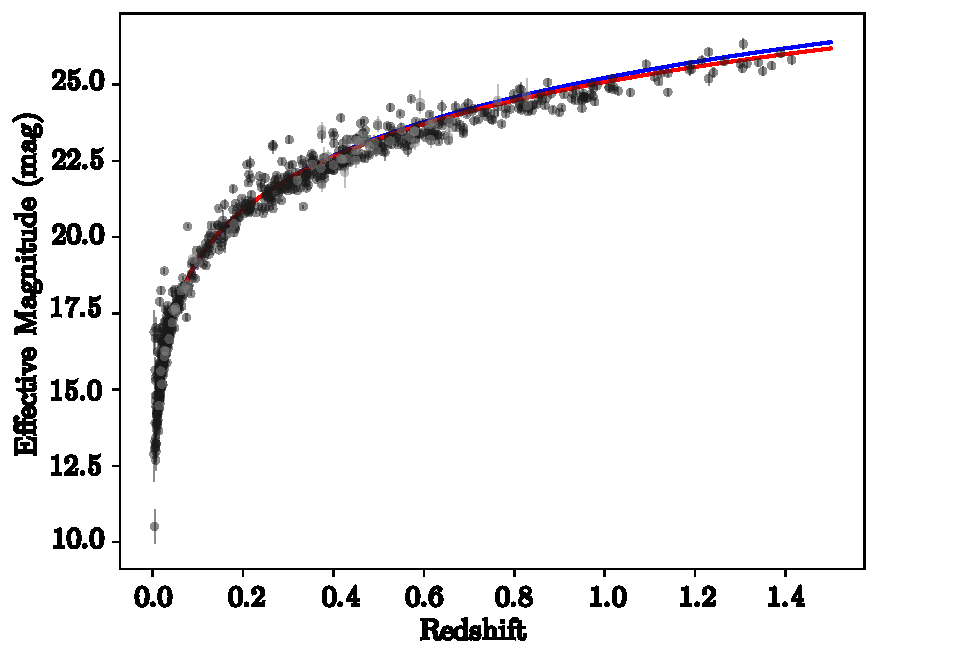
\includegraphics[width=9.25cm]{results/hubble_diagram}
\vspace{-3ex}
\caption[]{Hubble diagram showing the Union2.1 Type Ia supernova data plotted alongside two models. The blue line represents a universe with $\Omega_{\Lambda,1}=0.86\pm0.04$ and the red line $\Omega_{\Lambda,2}=0.74\pm0.01$. From reduced $\chi^2$ analysis the former parameter appears to be the best fit with $\chi^2_{\nu,1}=2.4539$ and $\chi^2_{\nu,2}=2.4547$ respectively. We note that there are too many points for the majority of magnitude error bars to be seen.}
\vspace{-3ex}
\label{fig:hubble_diagram}
\end{center}
\end{figure}

In Figure \ref{fig:hubble_diagram} we have plotted the Union2.1 data set alongside our two models which have been produced by using the calculated cosmological parameters from flux-space. To assess the quality of fit between the data and the model we have calculated reduced $\chi^2$ values. For the model which makes use of $\Omega_{\Lambda,1}=0.86\pm0.04$ we find $\chi^2_{\nu,1}=2.4539$, and for the secondary model which uses $\Omega_{\Lambda,2}=0.71\pm0.01$ we proceed to calculate $\chi^2_{\nu,2}=2.4547$. The criteria for a model to be a good fit to the data is to produce a reduced $\chi^2$ which is $\sim1$ \cite{hugheshase}. We therefore would be justified to conclude that $\Omega_{\Lambda,1}$ should be the accepted cosmological constant as it is a closer value to unity, even if it is not consistent with the literature value.  However, between both $\chi^2_\nu$'s there is only a $0.03\%$ difference and we can see from the figure that they are extremely similar. For that reason we could not form a convincing conclusion based on this analysis, instead we decided to explore Bayesian statistics in an attempt to see if the same results could be replicated and whether the accuracy could be improved.

\vspace{-3ex}
\subsection{Bayesian Statistics} 
\vspace{-2ex}
With our work in Bayesian statistics we have primarily made use of the Markov Chain Monte Carlo (MCMC) set of methods. Bayes theorem associates the posterior probability (the probability for parameters given known and observed data) to the likelihood (the probability for the data given certain parameters) and the prior (what was known about the parameter before the data). With these statistical procedures we are in essence updating our information about a value from the prior to the posterior \cite{mcmc_bs}. MCMC makes use of this theory and applies it into a methodology, values are generated and then assigned a likelihood probability, criteria is then used to decide if the parameters should be accepted or not, then finally an optimum solution should be found from all the runs.

For our use in constraining cosmological parameters we chose to utilise a Random Walk Metropolis-Hastings (RWHM) algorithm, the method for which can be found in Appendix \ref{appendix:mcmc}. We chose to use this as it independently samples the parameter space, information about it's current point will not be considered for the location of it's next `jump' \cite{mcmc_bs}. Instead, an acceptance probability and a random value is compared to generate the next point in the parameter search.

A more accurate value is therefore expected with the application of this algorithm. Although, we must first note that as this method relies on the random generation of new points, the optimum values will always lie within a range of $\sim 5\%$ above or below the literature values. To account for this, we therefore performed multiple runs of the algorithm and then averaged them together to find an acceptable value. 

To find solely $\Omega_\Lambda$ we carried out 10 runs of 1500 walks each, from this we found a value of $0.72\pm0.01$. Whilst this does agree with literature, we find that the number calculated with Least Squares is more accurate than what we have here. This could be the case due to the number of walks given to the algorithm in a single run, if 10,000 walks had been allocated could we have seen the optimum match more closely to what has been measured? There is a substantial problem with doing this, if left unaided the search could end up trapped in a `local minima' and it could take many walks before it is able to escape. 

In some of our experiments we became confined in these wells, one example is when we found $\Omega_\Lambda=0.47\pm0.02$, a value which is drastically different to what we have found previously. We can see in Figure \ref{fig:mcmc_search} the dynamics of what occurs. The red dot signifies the initial search parameters for each individual run, this is always $\Omega_\Lambda=0.80$ and $L_\text{peak}=3.40\times10^{35}$. All 10 of the runs have an optimum within the vicinity of $\Omega_\Lambda \approx 0.4$ and $\L_\text{peak}\approx2.9\times10^{35}$ which strongly suggests that a minima was encountered, plus the majority of the walks seems to have been contained within $1\sigma$ of the optimum average result further implying that it has been weighted towards a certain value.

\begin{figure}[!h]
\begin{center}
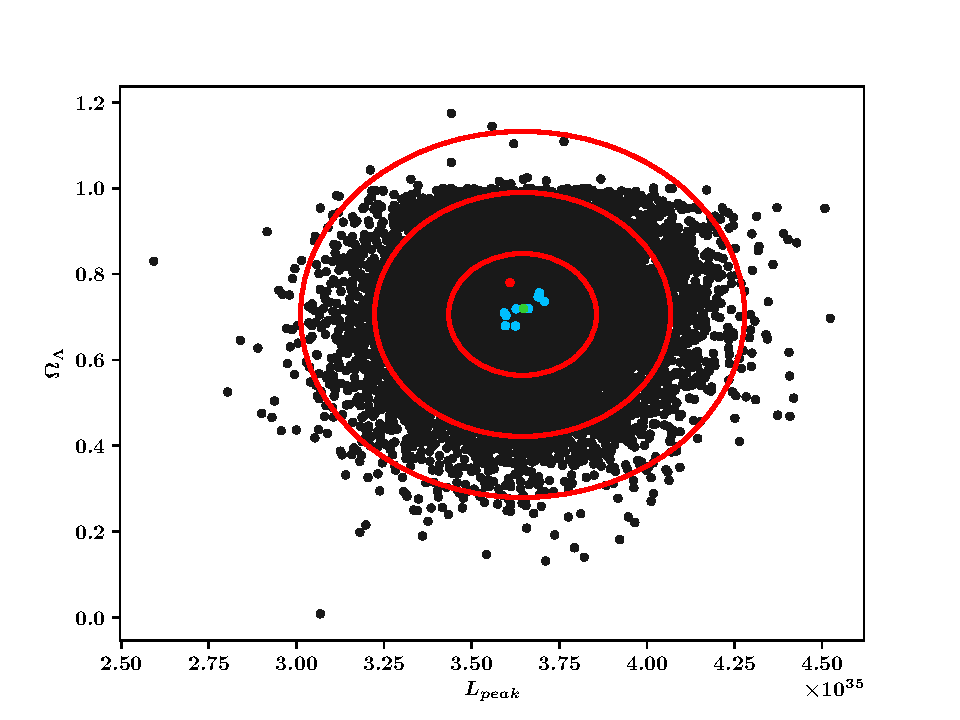
\includegraphics[width=9.25cm]{results/ol_lp_complete}
\caption[]{Random Walk Metropolis-Hastings algorithm shown when constraining $\Omega_\Lambda$ and $L_\text{peak}$. 10 independent runs performed with 1500 individual random walks for each run. The red dot is the initial provided search parameters $\Omega_\Lambda=0.8$ and $L_\text{peak}=3.40\times10^{35}$, the blue dots represent the optimums for each of the 10 runs, and the green dot is the final average of all of the optimum parameters from each run. The ellipses represent the spread of data with the inner ellipse as $1\sigma$, second as $2\sigma$, and the third as $3\sigma$. This plot shows us the potential for the algorithm to become stuck within local minima if left unconstrained. }
\vspace{-5ex}
\label{fig:mcmc_search}
\end{center}
\end{figure}

We can circumnavigate this problem by implementing \textit{simulated annealing}. This is where the descent algorithm is modified by random ascent moves so that local minima can be escaped \cite{simulated_annealing}. In our experimentation we did not apply these extra steps, instead we chose to avoid local minima by limiting the range of values that the cosmological values could take - we restricted the parameter space so it would not fall into any minima. 

\vspace{-3ex}
\subsection{Multi-cosmological Parameters} 
\vspace{-2ex}
With the knowledge that local minima could be encountered when performing these MCMC searches, we then decided to see how searching for multiple cosmological parameters would affect it. So, we required a more detailed model of the universe which would include extra variables into our testing. We therefore turned to the Lambda Cold Dark Matter model ($\Lambda$CDM) where a propotion of the universe is made up of cold dark matter and vacuum energy \cite{mod_ast, quintessence}. 

For the purpose of testing our search algorithms we decided to implement a larger equation which describes the cosmic expansion history $H(z)$, 
\begin{multline}
H(z)=H_0[X(z)\Omega_\Lambda+(1+z)^2\Omega_k+\\
(1+z)^3\Omega_m+(1+z)^4\Omega_r]^{1/2},
\label{eqn:expansion_history}
\end{multline}

where $X(z)$ is the dark energy density relative to its present value, $\Omega_k$ is the spatial curvature of the universe, and the other terms are as previously defined in Section \ref{sec:cosmo_parameters} \cite{cosmo_constraints}.

{\renewcommand{\arraystretch}{1.2}%
\begin{table}[h!]
\centering
\begin{tabular}{c@{\hskip 15pt}c@{\hskip 15pt}c} 
 \hline
 \textbf{Parameter} & \textbf{$\boldsymbol{X(z)=1}$} & \textbf{Literature} \\ [0.5ex] 
 $L_{\text{peak}}$ (W) & $(3.3\pm0.1)\times 10^{35}$ & - \\
 $\Omega_\Lambda$ & $0.76\pm0.04$ & $0.761^{+0.017}_{-0.018}$ \\
 $\Omega_k$ & $-0.002\pm0.001$ & $-0.0030^{+0.0095}_{-0.0102}$ \\
 $\Omega_m$ & $0.32\pm0.02$ & $0.239^{+0.018}_{-0.017}$ \\
 $\Omega_r$ & $(3.2\pm0.2)\times10^{-6}$ & $(4.16)\times10^{-6}$ \\
 \hline
\end{tabular}
\caption{We have calculated cosmological parameters using Equation \ref{eqn:expansion_history} with $X(z)=1$. We present the averaged results from our 10 runs of 100 steps each, we limited the search range available for the algorithm to avoid local minima. Literature values have also been provided for comparison. We conclude that we are able to produce consistent values inline with measured literature parameters.}
\vspace{-0.5em}
\label{table:extended_search}
\end{table}

Initially we chose to set $X(z)=1$ as this represents simple `vanilla dark energy' \cite{cosmo_constraints}, we believed that this would be a good starting point to test whether we could achieve values in the range of the literature numbers. Starting with the same conditions of 1500 walks for 10 runs we found that local minima would certainly be encountered, there would often be a $\sim 40\%$ difference between the generated values and literature. Whilst we originally had suggested that these wells could be escaped given a large enough number of steps, investigating the data sets for the entire run we find digressions occur more rapidly due which could potentially be attributed to the number of parameters that are being constrained. To allow for a reasonable and fair search we reduced the number of walks to the approximate point where digression occurs, $\sim100$ steps.  

In Table \ref{table:extended_search} we find the averaged results from 10 runs which used the 100 steps per run. Comparing with the literature values we find that our results are within range and in agreement. To decide whether to accept them as a formal result requires us to further analyse the data which is produced. One way we can do this is by calculating if there are any correlations between our generated parameters. We know that for some of our variables there should be a correlation, take $\Omega_\Lambda$ and $\Omega_m$, they are related through the total density parameter as given by Equation \ref{eqn:total_density}. Looking at the calculated correlation values in Table \ref{table:correlations} we find that they have no connection, $-0.105$. Correlation occurs at values of $-1$ or $1$, with $0$ representing no correlation. In fact, bar themselves, there appears to be little connection throughout the parameters.

Accordingly we must therefore remain skeptical in our results, whilst they appear to be in agreement with literature, with the issue of local minima at hand, more work such as implementing simulated annealing must be performed before we can accept our values. 

{\renewcommand{\arraystretch}{1.2}%
\begin{table}[h!]
\centering
\begin{tabular}{c@{\hskip 10pt}c@{\hskip 10pt}c@{\hskip 10pt}c@{\hskip 10pt}c@{\hskip 10pt}c} 
 \hline
  & \textbf{$\boldsymbol{L_\text{peak}}$} & \textbf{$\boldsymbol{\Omega_\Lambda}$} & \textbf{$\boldsymbol{\Omega_k}$} & \textbf{$\boldsymbol{\Omega_m}$} & \textbf{$\boldsymbol{\Omega_r}$} \\ [0.5ex] 
 \textbf{$\boldsymbol{L_\text{peak}}$} & +1.000 & $-0.088$ & +0.083 & $-0.213$ & $-0.250$ \\
 \textbf{$\boldsymbol{\Omega_\Lambda}$} & $-0.088$ & +1.000 & $-0.113$ & $-0.105$ & $+0.128$ \\
 \textbf{$\boldsymbol{\Omega_k}$} & +0.083 & $-0.113$ & +1.000 & $-0.107$ & $-0.108$ \\
 \textbf{$\boldsymbol{\Omega_m}$} & $-0.213$ & $-0.105$ & $-0.107$ & +1.000 & +0.004 \\
 \textbf{$\boldsymbol{\Omega_r}$} & $-0.250$ & $+0.128$  & $-0.108$ & +0.004 & +1.000\\
 \hline
\end{tabular}
\caption{Correlation values have been calculated for the $X(z)=1$ model data used to find the cosmological parameters as shown in Table \ref{table:extended_search}. Between the variables there is little correlation due to the independent random generation of them - correlation is found when the correlation value is $\sim1$ or $\sim -1$ \cite{hugheshase}.}
\vspace{-0.5em}
\label{table:correlations}
\end{table}

However, we then decided to further test this reduced number of walks. Therefore we left the $\Lambda$CDM framework and introduced the concept of \textit{quintessence}. With the Quintessence Cold Dark Matter model (QCDM) to explain the non-matter component which contributes to the total density parameter $\Omega=1$, a mixture of cold dark matter and quintessence is used, where quintessence is a slowly-varying and spatially-inhomogeneous component \cite{quintessence}. An equation-of-state $w$ can be attributed to account for the missing energy, with it being related to the negative pressure $p$ and the density of the energy $\rho$ through $w=p /\rho$. This can be incorporated into Equation \ref{eqn:expansion_history} by letting $X(z)=(1+z)^{3(1+w)}$ \cite{cosmo_constraints}. In QCDM we find $-1< w \leq 0$ and comparatively $w=-1$ for $\Lambda$CDM \cite{quintessence} which produces the previously defined simplification of $X(z)=1$.

Allowing our algorithm to now sample values for $w$ we find that the results for the other parameters seem to have improved in accuracy when compared to the earlier $\Lambda$CDM work. We can view in Table \ref{table:cosmo_parameters} that $w$ has just a $3\%$ difference between itself and it's literature value, with the other parameters similarly deviated. However we cannot conclude that more parameters means greater accuracy as this is more than likely due to the nature of the random walks. What we can draw from this then is that the altering of the number of parameters does have an effect on the constraining of cosmological variables, but there is a larger sensitivity to the number of walks used in the RWHM algorithm. 

$H_0$ and speed of light have been chosen, maybe choose different values for that 

\vspace{-3ex}
\subsection{Further Investigation} 
\vspace{-2ex}
Cosmic microwave background and baryons 


\vspace{-5ex}
\section{Conclusions}
\vspace{-2ex}

In conclusion, we have found that it is possible to constrain cosmological parameters of the universe using Type Ia supernova data.

In attempting to circumnavigate this problem \textit{simulated annealing} could be implemented. This is where the descent algorithm is modified by random ascent moves so that local minima can be escaped [[CITE]]. In our experimentation these minima were minimised by limiting the range of values that the parameters could take. However, for larger searches it would be highly useful if the sampling avoided becoming trapped as resources would be wasted in rerunning the algorithm.

\vspace{-3ex}
\bibliographystyle{abbrv}
\bibliography{supernova_cosmology}

\clearpage
\appendix

\vfill
\twocolumngrid
\vspace{-3ex}
\section{Uncertainties}
\vspace{-2ex}



\clearpage

\vspace{-3ex}
\section{Random Walk Metropolis-Hastings MCMC}
\label{appendix:mcmc}
\vspace{-2ex}

poo

\clearpage
\end{document}